\documentclass[a4paper]{article}
\usepackage[margin=0.4in]{geometry}
\usepackage[T1]{fontenc}
\usepackage[utf8]{inputenc}
\usepackage{lmodern}
\usepackage{amsmath}
\usepackage{amssymb}
\usepackage{geometry}
\usepackage{enumerate}
\usepackage{xcolor}
\usepackage{graphicx}
\usepackage{amsthm}
\newtheorem{theorem}{Theorem}[section]
\newtheorem{lemma}[theorem]{Lemma}
\newtheorem{corollary}[theorem]{Corollary}
\newtheorem{definition}[theorem]{Definition}
\usepackage{listings}
\usepackage{authblk}
\usepackage{titling}
\usepackage{zlmtt}
\usepackage{fancyvrb}
\usepackage[hidelinks]{hyperref}
\setlength{\droptitle}{-2em}
\lstset{frame=tb,
  language=C,
  aboveskip=3mm,
  belowskip=3mm,
  showstringspaces=false,   
  columns=flexible,
  basicstyle={\small\ttfamily},
  numbers=none,
  numberstyle=\tiny\color{gray},
  keywordstyle=\color{blue},
  commentstyle=\color{brown},
  stringstyle=\color{orange},
  breaklines=true,
  breakatwhitespace=true,
  tabsize=3
}
\begin{document}
\title{CS3210 Lab 1 Report}
\author{
  Wang Xiyu, Sun Weiyang (discussed with)
}
\maketitle
\par\vspace{-2em}
\section{Code Overview}
\par\vspace{-0.5em}
The provided code describes the bubble sort algorithm which is known to be sub-optimal ($\Theta(n^2)$).
This function sorts an array by comparing every pair of values in the array, and swap when out of order.
A random large array generation utility function and the main function to test the program are also included. These are out of the scope of discussion.
\par\vspace{-1em}
\section{Performance}
\par\vspace{-0.5em}
At \texttt{ARRAY\_SIZE = 100000}, \texttt{MAX\_VALUE = 100000}, the time statistic from running \texttt{/usr/bin/time ./asdf} is as such:
\begin{lstlisting}
    Command being timed: "./asdf"
    User time (seconds): 71.48
    System time (seconds): 0.00
    Percent of CPU this job got: 99%
    Elapsed (wall clock) time (h:mm:ss or m:ss): 1:11.49
\end{lstlisting}
\noindent
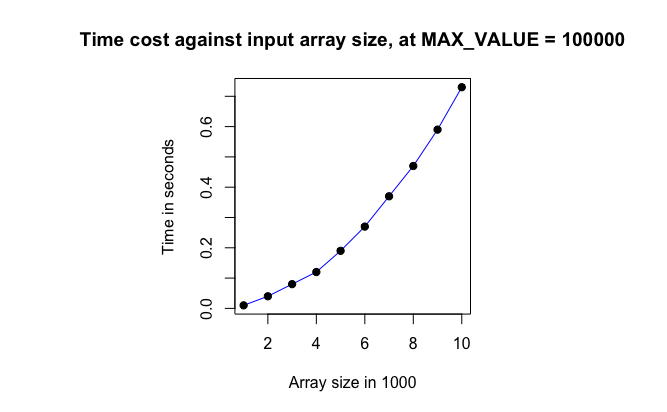
\includegraphics[width=0.49\columnwidth]{000030.png}%
\hfill
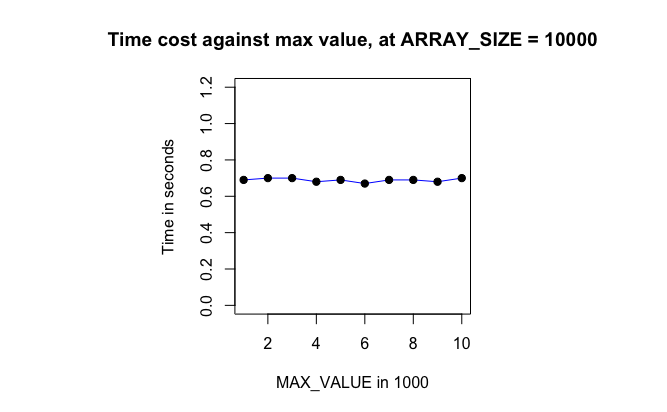
\includegraphics[width=0.49\columnwidth]{000058.png}
It's observed that the time growth in a quadratic manner as the array size increases, align with the common knowledge that bubble sort has a time complexity of $\Theta(n^2)$.\\
It's also observed that \texttt{MAX\_VALUE} has no substantial impact on the performance.
\par\vspace{-1em}
\section{Optimization}
\par\vspace{-0.5em}
\subsection*{Performance bottleneck}
\texttt{\$ flamegraph -- ./asdf "10000"} yields flamegraph as shown below:\\
\noindent\makebox[\columnwidth][c]{%
  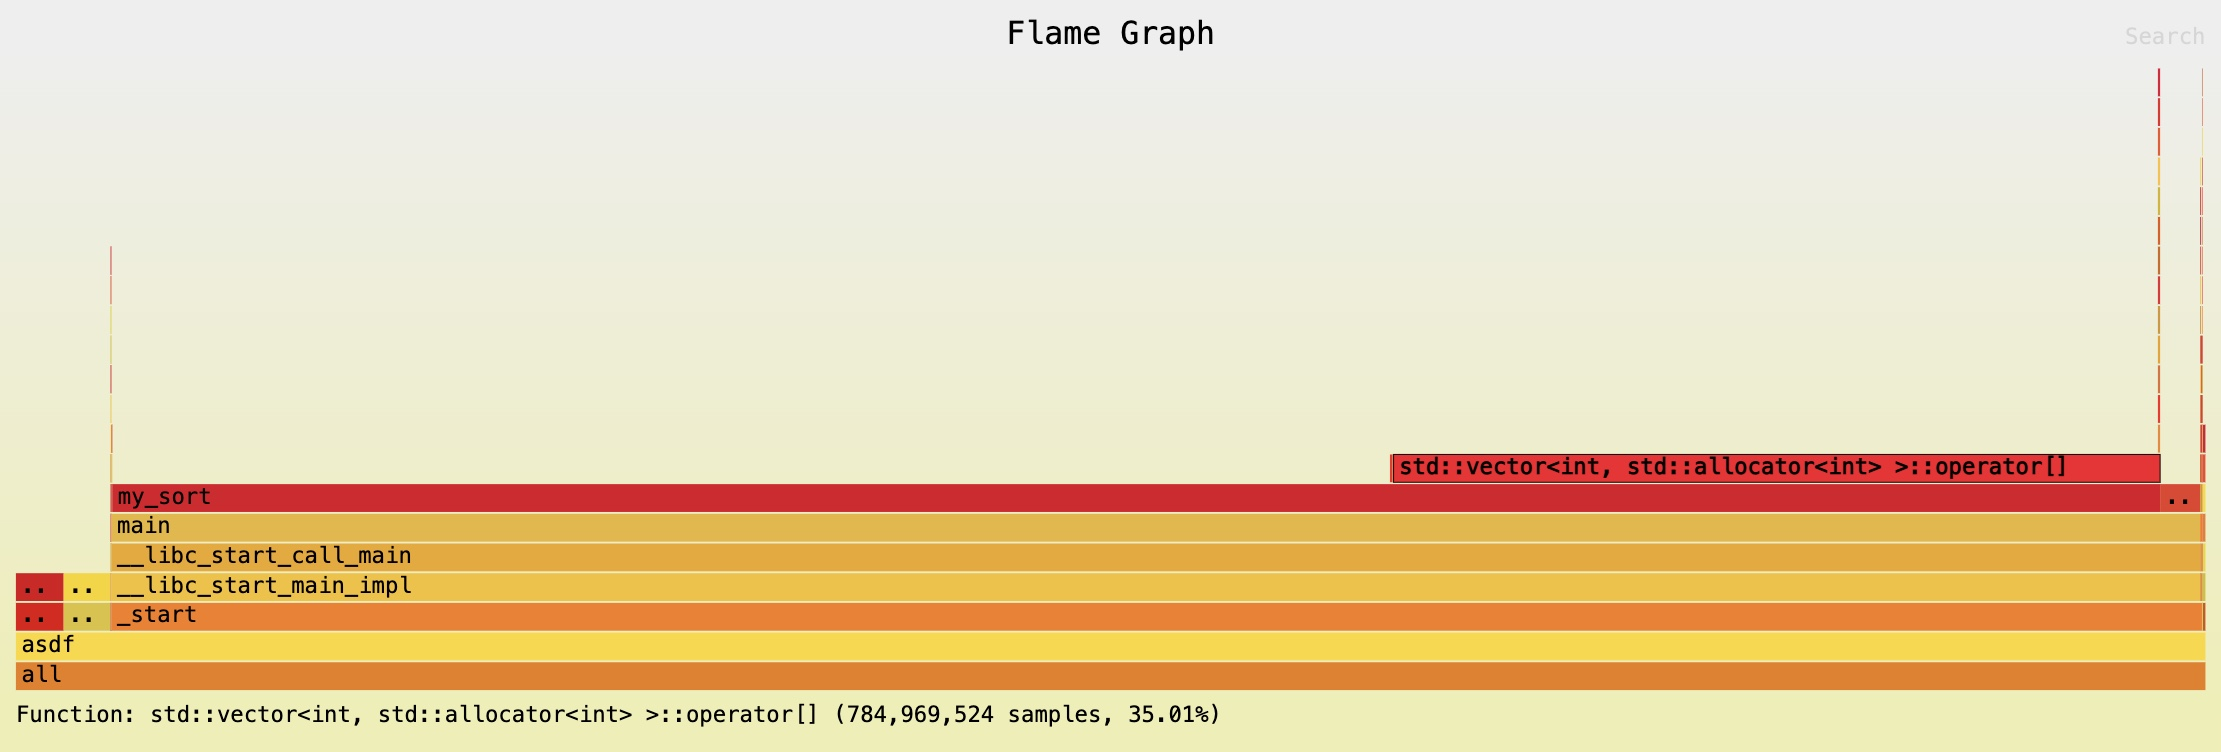
\includegraphics[
    width=\columnwidth,
    trim=0 0 0 0,
    clip
  ]{flg.jpeg}
}
Since we do not focus on improve the algorithm, we foucs on the overhead named 
\texttt{std::vector<int, std::allocator<int> >::operator[]},
 which is the cost associated with access elements in \texttt{vector} container, within \texttt{my\_sort()} function call.
\begin{lstlisting}
    $ perf record -- ./asdf 10000
    $ perf report
    Overhead  Command  Shared Object         Symbol
     61.23%   asdf     asdf                  [.] my_sort(std::vector<int, std::allocator<int> >&)
     38.32%   asdf     asdf                  [.] std::vector<int, std::allocator<int> >::operator[](unsigned long)
\end{lstlisting}
\subsection*{Hypothesis and Implementation}
We hypothesize that this overhead caused by accessing the internal array elements of a vector can be optimized by accessing via pointers directly. Although doing so does not change the asymptotic 
order of growth, the saved random access constant overhead would have significant performance improvement for large $n$ in practice.
\par\vspace{3ex}
\begin{minipage}{0.45\linewidth}
    \begin{Verbatim}[frame=topline,numbers=left,label= Original,framesep=3mm]
void my_sort(std::vector<int>& array) {
    size_t n = array.size();

    for (size_t i = 0; i < n - 1; ++i) {
        for (size_t j = 0; j < n - i - 1; ++j) {


            if (array[j] > array[j + 1]) {
                int temp = array[j];
                array[j] = array[j + 1];
                array[j + 1] = temp;
}}}}
    \end{Verbatim}
    \end{minipage}\hfill
    \begin{minipage}{0.45\linewidth}
    \begin{Verbatim}[frame=topline,numbers=left,label= Optimized,framesep=3mm]
void my_sort_o(std::vector<int>& array) {
    size_t n = array.size();
    int* init_ptr = array.data();
    for (size_t i = 0; i < n - 1; ++i) {
        for (size_t j = 0; j < n - i - 1; ++j) {
            int* cur = init_ptr + j;
            int* nxt = cur + 1;
            if (*cur > *nxt) {
                int t = *cur;
                *cur = *nxt;
                *nxt = t;
}}}}
    \end{Verbatim}
    \end{minipage}\hfill
\section{Reproduce result}
Compile the original code \texttt{asdf.cpp} and optimized version \texttt{asdfo.cpp}, 
\begin{lstlisting}
    g++ -g -o asdf asdf.cpp
    g++ -g -o asdfo asdfo.cpp
\end{lstlisting}
Run \texttt{./time\_test.sh} with custom steps and \texttt{ARRAY\_SIZE} and 
check \texttt{res.txt} and \texttt{res\_o.txt} for runtime log.
\par\vspace{-1em}
\section{Performance measurement}
\par\vspace{-1.5em}
\par\vspace{3ex}
\begin{minipage}{0.5\linewidth}
    \noindent\makebox[\columnwidth][c]{%
    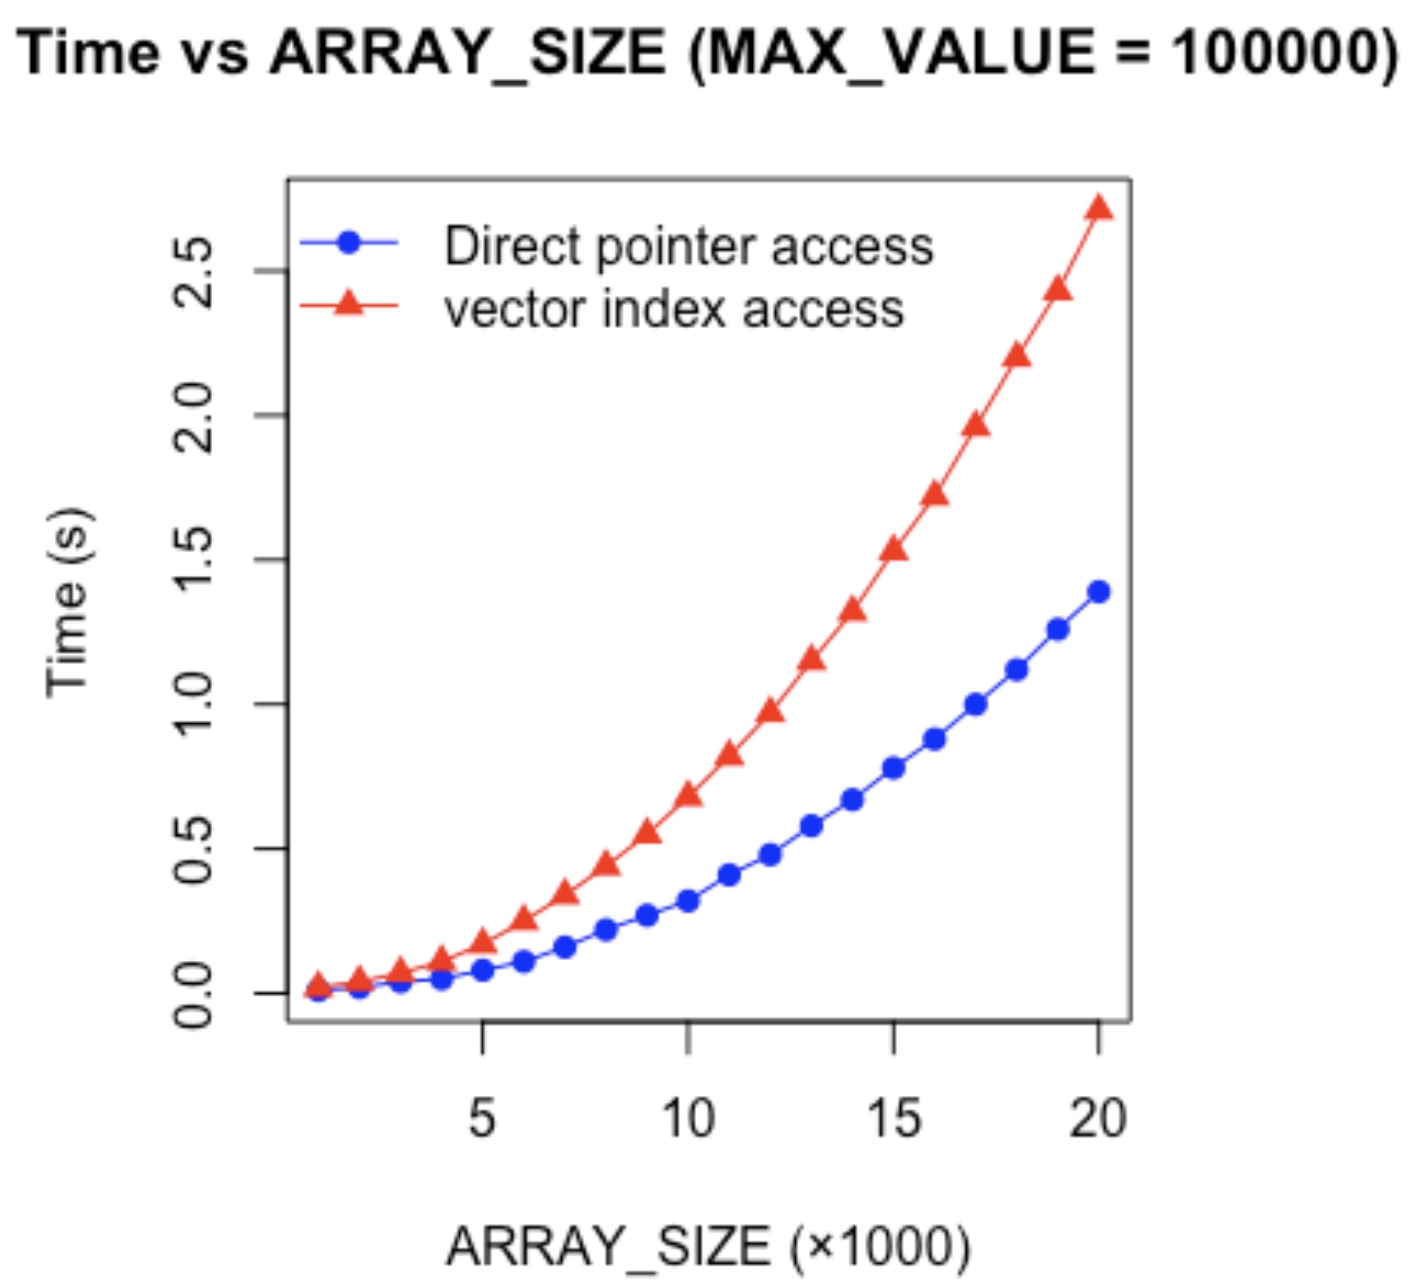
\includegraphics[
      width=\columnwidth,
      clip
    ]{comp.jpeg}
  }
    \end{minipage}\hfill
    \begin{minipage}{0.5\linewidth}
        We can see at large $n$ ($n \geq 10000$), the optimzed version has $\sim 50\%$ decrease in runtime, while retaining quadratic increasing trend,
        which proves our hypothesis that the constant access cost of vector element can be optimized.
    \end{minipage}\hfill
    \par\vspace{3ex}

\section{Appendix}
All resources used in preparing the diagrams, e.g. scripts, modified code can be found here: 
\href{https://github.com/Wxy2003-xy/CS3210-Lab-References}{Link}
\end{document}
